\subsection{Messverfahren}
Die Versuchsaufbauten wurden mithilfe eines Steckbretts und den elektronischen Bauteilen flexibel realisiert. Ein digitaler Funktionengenerator speiste die Schaltungen mit dem gewünschten Signal, während die Ausgangsspannungen jeweils direkt an den relevanten Schaltungspunkten erfasst und mithilfe eines digitalen Oszilloskops ausgewertet wurden. Die Steuerung beider Geräte erfolgte über eine zentrale PC-Software. 
Für detaillierte Versuchsanleitungen ist das Skript\autocite{Skript_2.2} zu konsultieren.
\paragraph{Aufgabe 1}
Die Halbwertszeiten verschiedener RC-Glieder werden mithilfe der Cursorfunktion des Oszilloskops vermessen. Dazu wird in Kanal 1 die Spannung über den Kondensator abgenommen, in Kanal 2 die Eingangsspannung angezeigt. Anschließend wird die Spannung einmal über dem Widerstand abgegriffen, die nach \(U_R=RI\) dem Strom im RC-Glied entspricht. Somit kann überprüft werden, ob die Halbwertszeit des Stromverlaufs die gleiche ist. 
\paragraph{Aufgabe 2}
Als nächstes wird ein RC-Glied als Integrator/Differentiator verwendet, es werden verschiedene Signalformen ausgesendet und mithilfe des Integrators/Differentiators umgewandelt. Die resultierende Ausgangsspannungsform wurde protokolliert.  
\paragraph{Aufgabe 3}
Der Frequenz- und Phasengang eines Tiefpass- bzw. Hochpassfilters werden aufgenommen. Mithilfe des Cursors wird die Grenzfrequez bestimmt. 
\paragraph{Aufgabe 4}
Ein Serienschwingkreise mit einem variablen Widerstand wird genutzt, um jeweils die Resonanzfrequenz, die Bandbreite und den Effektivwert der Ausgangsspannung (über dem Widerstand) aus dem Frequenzgangsbild zu bestimmen. Die Amplitude der Eingangsspannung kann
am Oszilloskop abgelesen werden.
\paragraph{Aufgabe 5}
Als nächstes untersuchen wir das Phänomen der Resonanzüberhöhung. Der Serienschwingkreis mit konstantem Widerstand der vorherigen Aufgabe wird verwendet, um nun den Frequenzgang über jedem Bauteil aufzunehmen. Aus dem Diagramm werden mithilfe der Cursor die jeweiligen Resonanzfrequenzen über die Maxima der Amplitudenmessung ausgemessen.
\paragraph{Aufgabe 6}
Zur Untersuchung der Dämpfung des Schwingkreises wird der dämpfungsbedingte Abfall der Ausgangsspannung über der Spule aufgenommen. Dazu wird ein Rechtecksignal mit kleiner Frequenz (\(\omega\ll\omega_R\)) angelegt und die Frequenz notiert, bei der ein solcher Abfall schön zu sehen ist. Es wird der Spannungsabfall pro Periode gemessen, um daraus die Dämpfungskonstante zu bestimmen.  
\paragraph{Aufgabe 7}
Der Frequenzgang eines Parallelschwingkreis (Bandpassfilter) wird aufgenommen und daraus die Resonanzfrequenz bestimmt. Hierzu wird die Ausgangsspannung über dem Widerstand abgegriffen. 
\paragraph{Aufgabe 8}
Ein (gestörtes) Eingangssignal dreier sich überlagender Sinussignale soll mithilfe verschiedener Filterschaltungen aufbereitet werden. Zuerst wird das ungefilterte Signal dazu mithilfe der Fast-Fouriertransformation auf seine Bestandteile untersucht und im Folgenden jeweils die Fourierdarstellung (Fast-Fourier-Transformation FFT) (Spectrum Analyzer) und das Oszilloskopbild der Filterschaltungen gespeichert, aus dem FFT-Bild wird jeweils die Amplitude der drei Grundfrequenzen abgelesen. Als Filter werden nacheinander ein RC-Hochpassfilter, ein RC-Tiefpassfilter, ein LC-Tiefpassfilter und Bandpassfilter vorgeschaltet. 
\vfill
\subsection{Messprotokoll}
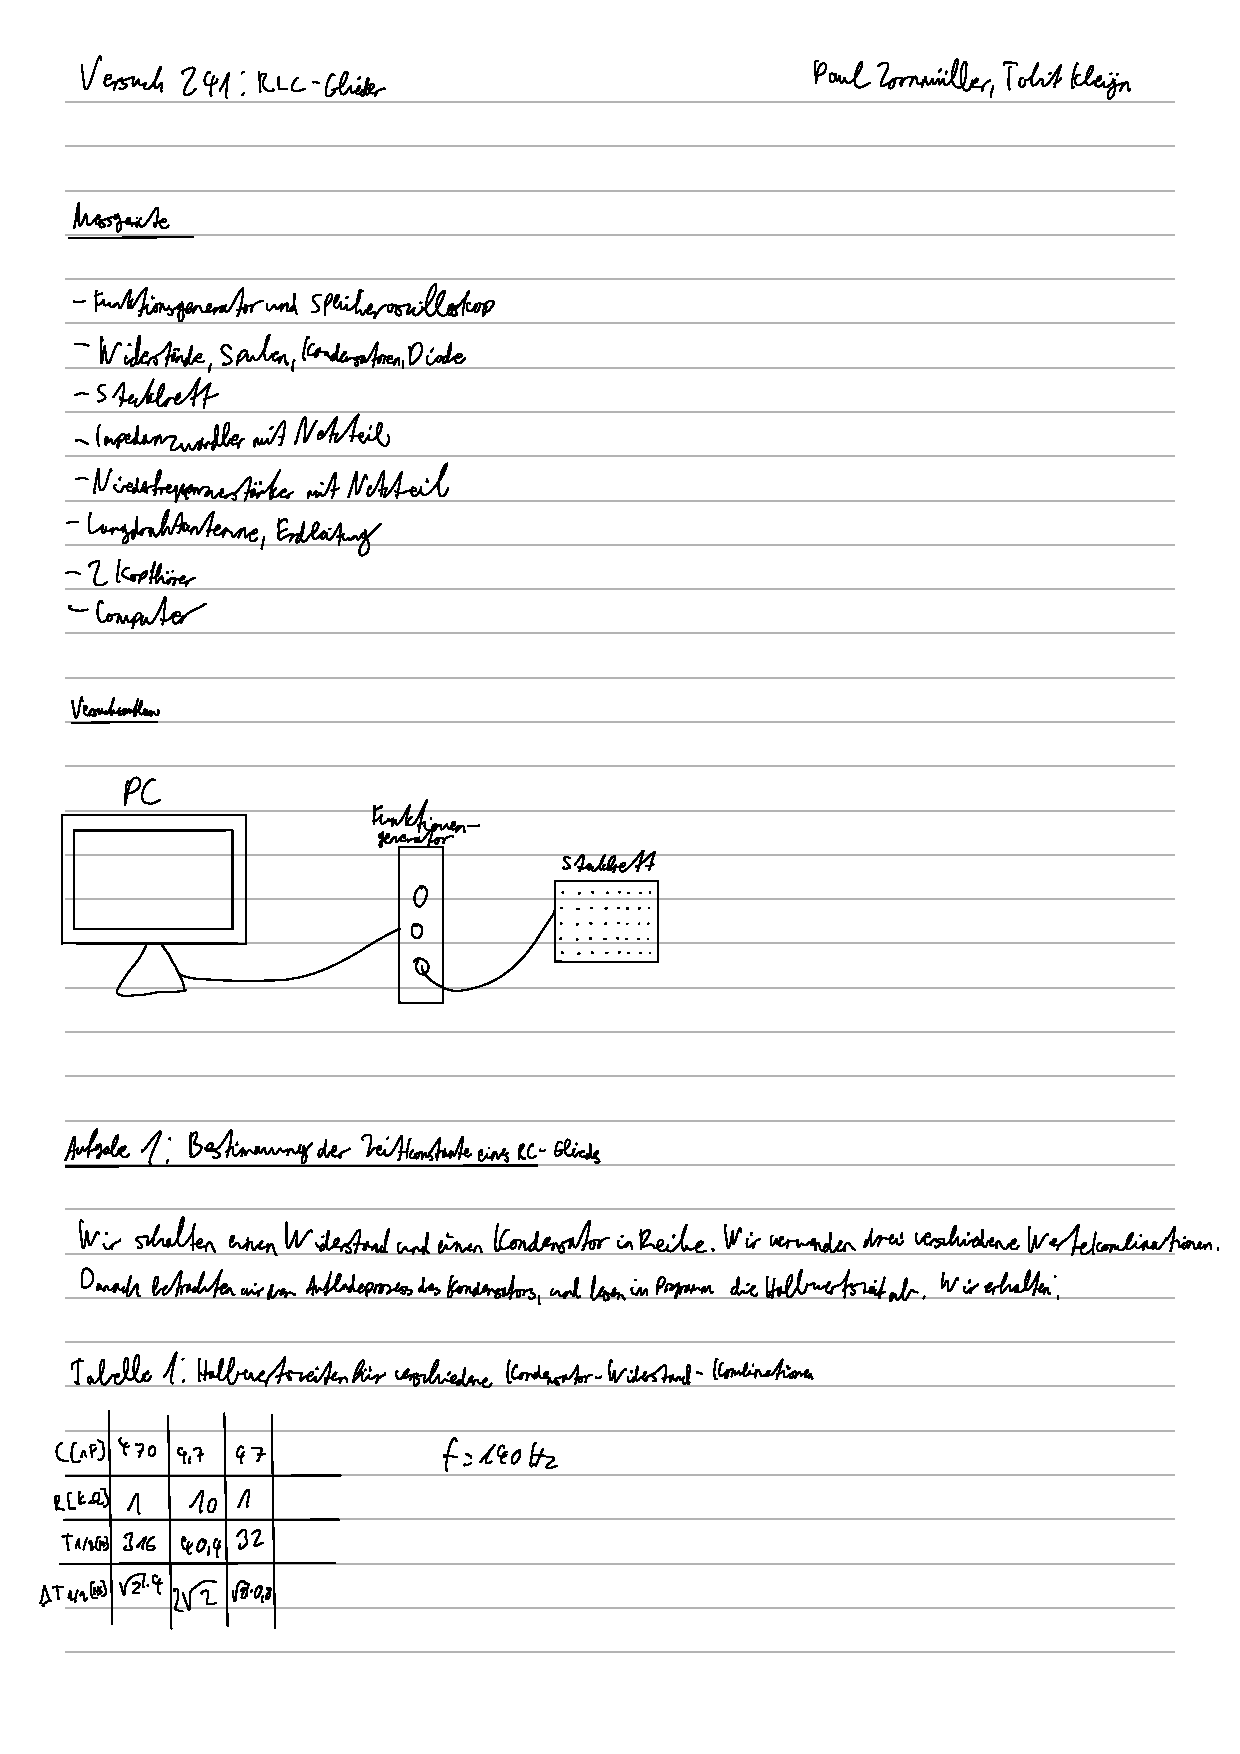
\includepdf[pages=-]{./images/241.pdf}
% heibox.uni-heidelberg.de/d/a48f9d7b91264990a16e/
